\section{Multicore Systems}
Since the limit of Frequency/Area (Power/Area) is reached.
The only performance increase for a giving area is by adding cores to the silicon design.
To make use of this potential performance increase, software must be designed for the use of multicores.
This is achieved if the Task are 100\% independent.
However some software is so performance hungry that is should be split up in parts if:
serial/sequential executed code and code that can be executed in parallel.

\subsection{Parallelism vs. Concurrency}
\columnratio{0.5}
\begin{paracol}{2}
    The source of software design for multicores is the computer science domain.
    Concurrency is not the same as parallelism.

    Simplest distinction is that concurrency is that different flows/tasks that run seemingly in parallel by interrupting on one core by interrupting each other.
    Parallelism is the case where the flows run each on separate cores.
    However parallelism is software design manner is when a application especially a task is split up into smaller tasks which can run in parallel on several cores.
    \switchcolumn
    \vspace{-1.5cm}
    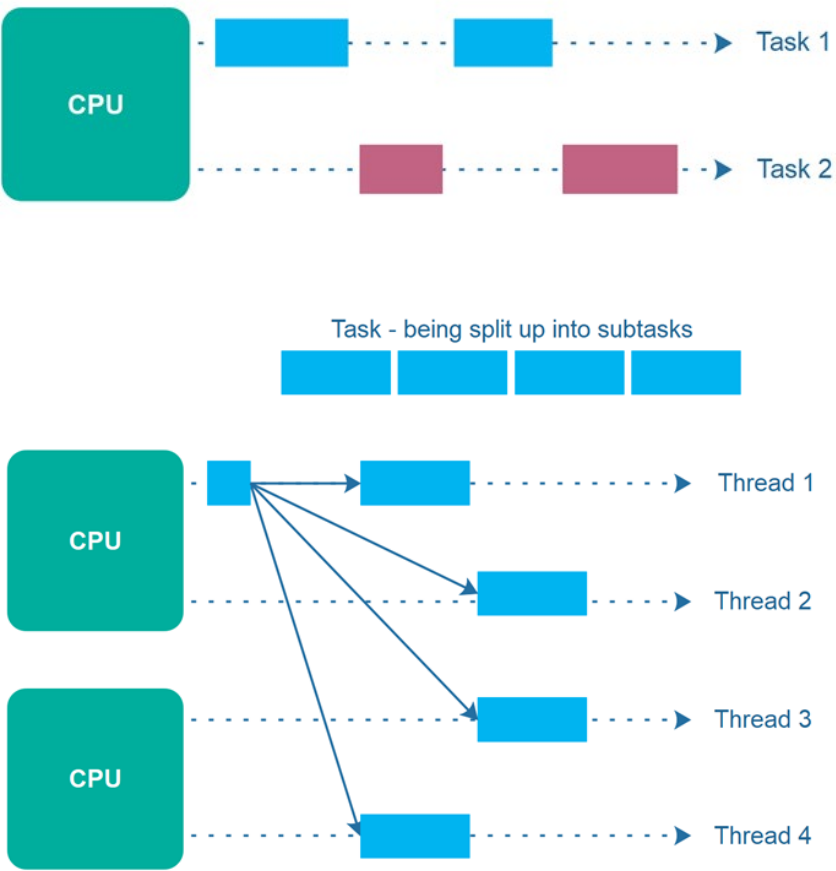
\includegraphics[width=0.4\textwidth]{images/Multicore/parallel_vs_concurrent.png}
\end{paracol}

\subsection{Key Challenges}
The following challenges are true for symmetric and asymmetric multicore platforms
\begin{itemize}
    \item Finding enough parallelism
    \item Achieving the right level granularity
    \item Exploiting locality in computation
    \item Proper load balancing
    \item Coordination and synchronization
\end{itemize}

\subsection{Adamahls Law}
In computer architecture, Amdahl's law is a formula which gives the theoretical speedup in latency of the execution of a task at fixed workload that can be expected of a system whose resources are improved. (1967)
Amdahl's law is often used in parallel computing to predict the theoretical speedup and is considered as pessimistic..
\begin{align*}
    S_\text{latency}(s) = \dfrac{1}{(1-p) + \frac{p}{s}}
\end{align*}
\begin{itemize}
    \item $S_\text{latency}$ is the theoretical speedup of the execution of the whole task
    \item $s$ is the speedup of the part of the task that benefits from improved system resources
    \item $p$ is the proportion of execution time that the part benefiting from improved resources originally occupied
\end{itemize}
\subsubsection{Extension by adding the Influence of Overhead}
Parallelism overhead comes from areas such as:
\begin{itemize}
    \item Overhead from starting a thread or process
    \item Overhead of communicating shared data
    \item Overhead of synchronizing
    \item Overhead from extra (redundant) computation required to parallelize some parallel algorithms
\end{itemize}
By introducing the new parameter, the curve no longer converges towards T/ts, but reaches a maximum, only to fall off again behind it.

This effect is also observed in practice:
With a sufficiently large number of processors, the effort to transmit, synchronize and send back the problem exceeds the computational effort that is taken away by the additional cores.
Formula extended and operands replaced with their ISO 8000 equivalents
\begin{align*}
    \eta_s = \dfrac{T}{t_S + t_{O(n_P)} + \frac{t_P}{n_P}} \leq \frac{T}{t_S} = \frac{T}{T-t_P}
\end{align*}
\begin{multicols}{2}
    \begin{itemize}
        \item $\eta_S$ Speedup factor
        \item $T$ Total runtime
        \item $t_S$ Runtime of serial part
        \item $t_P$ Runtime of parallel part
        \item $n_P$ Number of cores to be used in parallel part
        \item $t_{O(n_P)}$ Runtime for synchronization
    \end{itemize}
\end{multicols}

\subsection{Gustafsons' Law}
Gustafsons's Law defines the scope of the evaluation where the code runs in parallel.
Another assumption is that the overhead of synchronisation and start-up code will always a very small part of the parallel computing part.
Therefore a almost linear behaviour is the result of the formula of Gustafson’s law.
\begin{align*}
    S(N) = (1-P) + N\cdot P
\end{align*}
$P$ = parallel part, $N$ = number of cores.

Either of the two (Amdahls or Gusfason's) could apply to a particular Situation depending on the software design and application.

\subsection{Granularity}
Granularity can be described as the ratio of computation to communication in a parallel program.
Fine-grained parallelism implies partitioning the application into small amounts of work done leading to a low computation to communication ratio.
Coarse-grained parallelism is where there is a high computation to communication ratio.

\subsection{Data Dependency}
Not only code / logic can be parallelized.
Data is often used and data can be a limitation or a leverage to realise parallelism.
Dependencies between data reads and writes determine the partial order of computation.
There are three types of data dependencies which limit the ordering:
\begin{description}
    \item[True data dependencies] (read after write RAW) imply an ordering between operations in which a data value may not be read until after its value has been written.
          These are fundamental dependencies in an algorithm, although it might be possible to refactor algorithms to minimize the impact of this data dependency.
    \item[Antidependencies[] (write-after-read WAR) have the opposite relationship and can possibly be resolved by variable renaming.
          In an antidependency, a data value cannot be written until the previous data value has been read.
    \item[Output dependency] (write-after-write WAW) writes to a variable may not be reordered if they change the final value of the variable that remains when the instructions are complete.
\end{description}
\begin{itemize}
    \item Data dependencies fundamentally order the code
    \item Discuss three main types
    \item Analyze code to see where critical dependencies are and if they can be removed or must be honored
    \item Parallel dependencies are usually not so local - rather between tasks or iterations
\end{itemize}

\subsection{Parallelisation}
\subsubsection{Architecture Approaches}
\begin{description}
    \item[Decomposition:] consider how the application can be decomposed into task and data parallelism
    \item[Dependency analysis:] consider both control and data dependences
    \item[Design evaluation:] look at the suitability for the target platform
    \item[Design quality] consider what quality factors are important; performance, reliability, security, etc.
\end{description}

\subsubsection{Patterns}
\columnratio{0.6}
\begin{paracol}{2}
    \textbf{Master/Worker:} One master thread executes code sequentially until it reaches an area that can be parallelized.
    The master then triggers a number of worker threads to perform the parallel computational intensive work.
    Once computed, the worker threads turn the result back to the master and wait for additional work.\newline
    \switchcolumn
    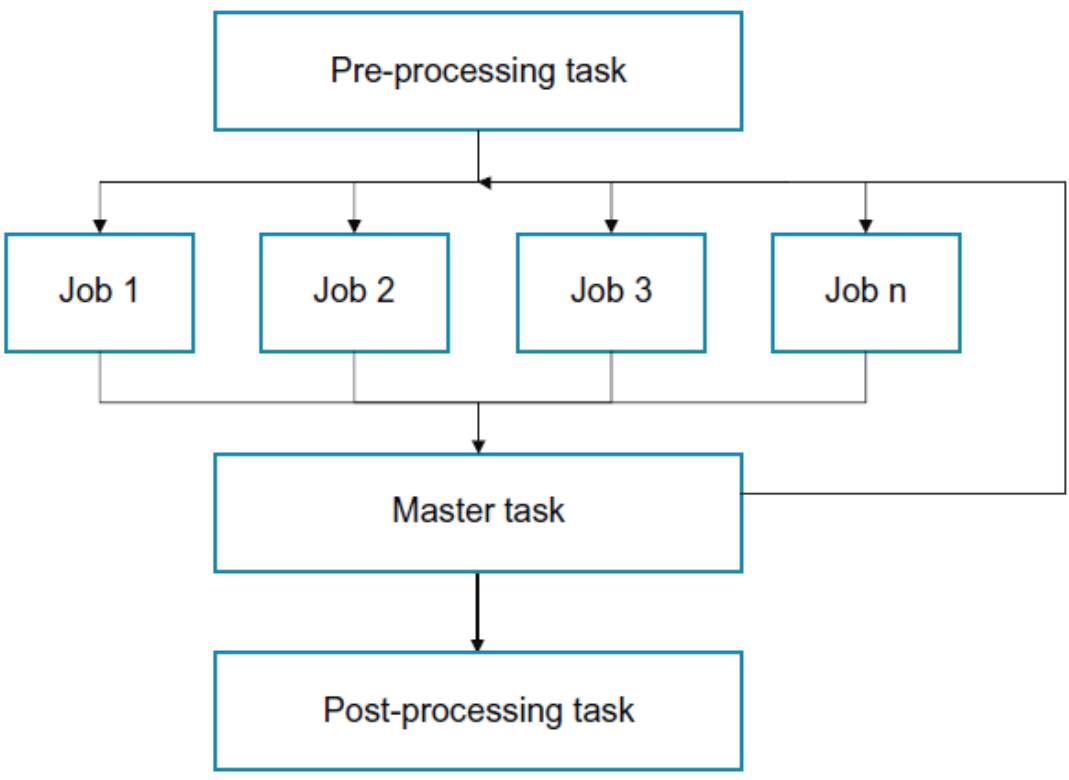
\includegraphics[width=0.3\textwidth]{images/Multicore/master_worker}
\end{paracol}

\begin{paracol}{2}
    \textbf{Peer:} This software architecture is similar to the master/worker pattern with the master also functioning as peer (worker) and shares the computational work.
    This approach can save a thread of execution.\newline
    \switchcolumn
    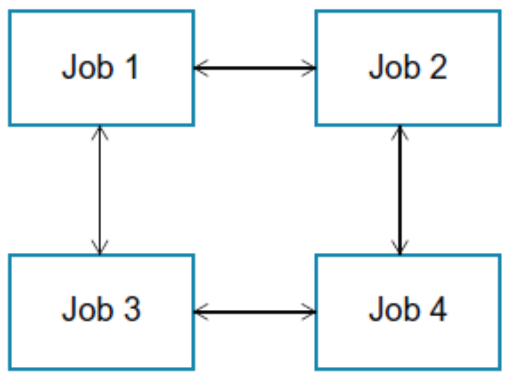
\includegraphics[width=0.16\textwidth]{images/Multicore/peer}
\end{paracol}

\begin{paracol}{2}
    \textbf{Pipelined:} A pipelined architecture involves dividing the applications into a series of smaller, independent stages.
    The output of one stage is the input to the next stage.
    Each one of the stages can be placed on a seperate core.
    This forms a series of decoupled stages in the pipeline.
    These stages could be different protocol stack layers or specific functions such as encryption/decryption
    \switchcolumn
    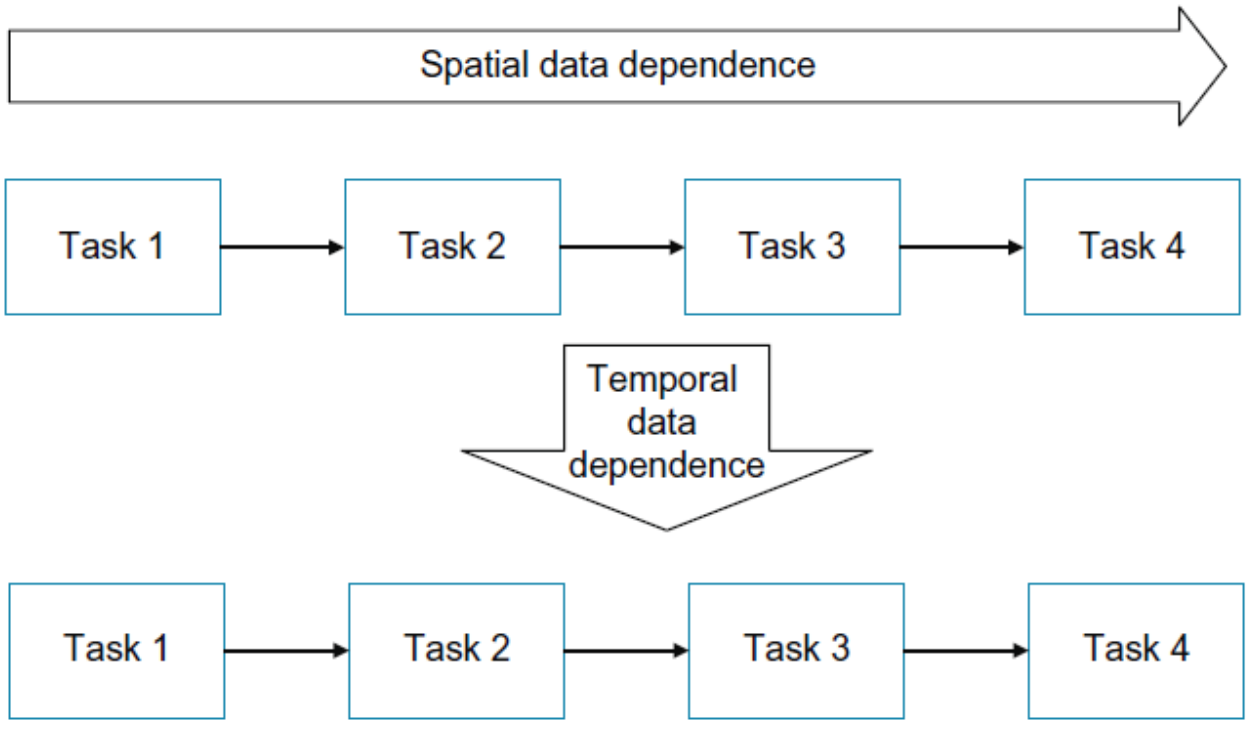
\includegraphics[width=0.4\textwidth]{images/Multicore/pipelined}
\end{paracol}

\subsection{Interprocessor Communication and Resource Managment in asynmetric Designs}
For Resource sharing and IPCC the IPCC and Resource management in asymmetric designs is realized by introducing solution from the symmetric core software solution domain:
Shared memory, pipes, semaphores into hardware solution (silicon).

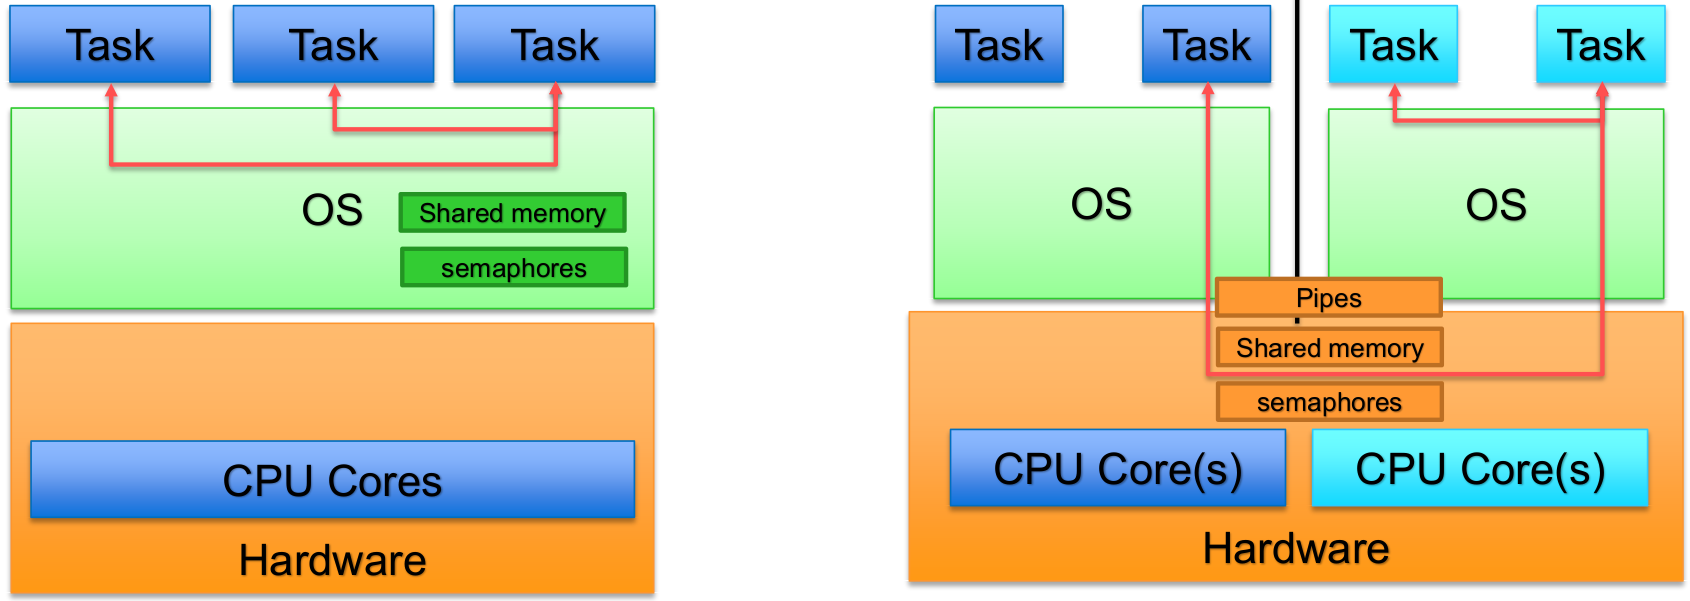
\includegraphics[width=0.8\textwidth]{images/Multicore/sharing_multi.png}

\subsubsection{Inter Processor Communication Controller (IPCC)}
\begin{table}[h]
    \begin{tabularx}{\textwidth}{lXX}
        \hline
        Manufacturer       & ST                                                                         & NXP                                                  \\\hline
        Peripheral name    & Inter Processor Communication Controller (IPCC)                            & Messaging Unit (MU) (imx6sx, imx7s, imx8qxp, imx8qm) \\
        Nubmer of channels & 6                                                                          & 4 (4x4 wires)                                        \\
        Message storage    & shared memory                                                              &                                                      \\
        Software library   & STMP151\newline M4: IPCC HAL driver C,\newline A7: Linux mailbox framework & FreeRTOS/Linux RPMsg                                 \\
        Exception          & STM32H7: shared memory                                                     &                                                      \\\hline
    \end{tabularx}
\end{table}

\columnratio{0.5}
\begin{paracol}{2}
    \begin{itemize}
        \item The message process is similar to communication via UART.
        \item ST offers various hardware-based solutions.
        \item NXP offers libraries that are based on operating systems and then use the hardware.
    \end{itemize}
    \switchcolumn
    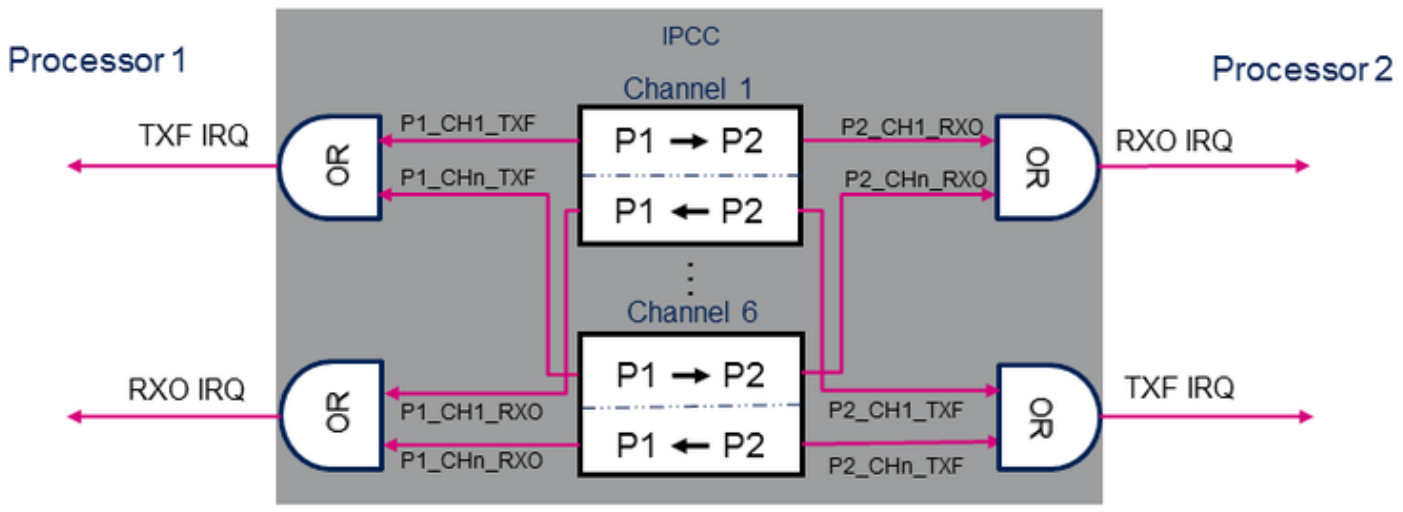
\includegraphics[width=0.5\textwidth]{images/Multicore/ipcc.png}
\end{paracol}

\paragraph{IPCC STM32H7 with FreeRTOS}
In FreeRTOS the message and stream buffer were introduce in V10.
These buffers can be mapped on shared memory domains of the STM32H7.
The mapping is performed by defining the buffer in MessageBufferAMP.h (\texttt{.../FreeRTOS\_AMP\_Dual\_RTOS/Common/Inc}).

Consequently, the code is in both cores CM4 and CM7.
See \texttt{xControlMessageBuffer} in main.c of CM4 and CM7

Three other hardware elements can be used for IPCC which are not mapped to FreeRTOS:
\begin{description}
    \item[Hardware semaphore HSEM]
    \item[EXTI controller and send-event instruction:] A notification mechanism by simply executing the SEV (send-event instruction).
    \item[DMAs and MDMA:] The DMA memory to memory mode work as a transfer channel to copy data from one CPU SRAM buffer to a shared buffer (intended for CPU2), and the transfer-complete interrupt can be used to notify CPU2 that new data was written into the shared buffer.
          This will offload the CPU and with more than two DMA controllers available in the product, dedicated channels can be defined during application resource partitioning to perform inter-processor communication.
\end{description}

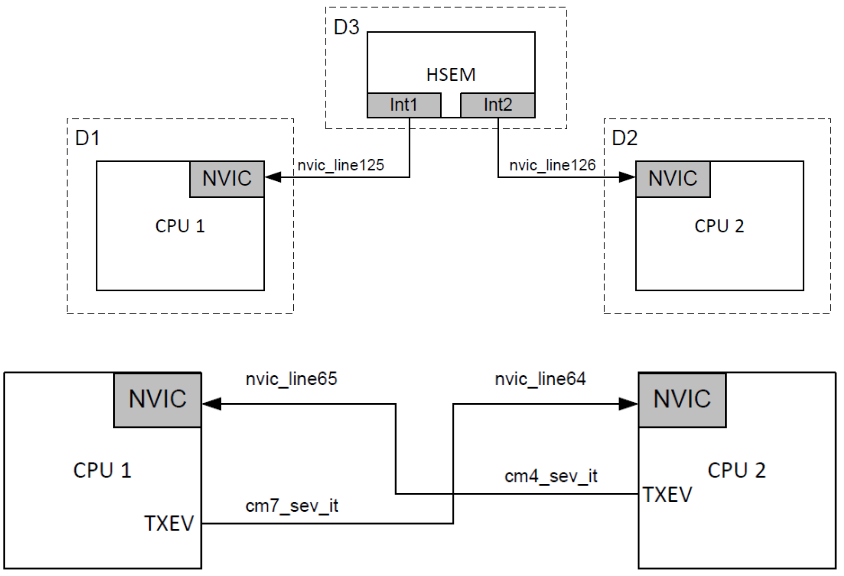
\includegraphics[width=0.55\textwidth]{images/Multicore/hsem_nvic.png}

\subsubsection{Resource Assignment}
\begin{table}[h]
    \begin{tabularx}{\textwidth}{lXX}
        \hline
        Manufacturer               & ST                                                         & NXP                                             \\\hline
        Peripheral name            & Memory Protection Unit (MPU)                               & Resource Domain Controller (i.MX7 XRDC)         \\
        Independent memory regions & 8/16                                                       & 16                                              \\
        Overlapping                & possible                                                   & yes                                             \\
        Software library           & M4: IPCC HAL driver C,\newline A7: Linux mailbox framework & MCUXpresso SDK                                  \\
        Exception                  & MPU defines only memory assignment                         & Memory, Resources, security regions and domains \\\hline
    \end{tabularx}
\end{table}

\subsubsection{Hardware Semaphore}
\begin{table}[h]
    \begin{tabularx}{\textwidth}{lXX}
        \hline
        Manufacturer         & ST                                                                  & NXP                    \\\hline
        Peripheral name      & HSEM                                                                & SEMA42 (SEMA4 i.MX6-7) \\
        Number of semaphores & 32                                                                  & 16                     \\
        Lock mechanisms      & 2 (1 step, 2 step)                                                  & 1                      \\
        Software library     & MX: MPU HAL driver C,\newline A7: Linux hardware spinlock framework & MCUXpresso SDK         \\\hline
    \end{tabularx}
\end{table}
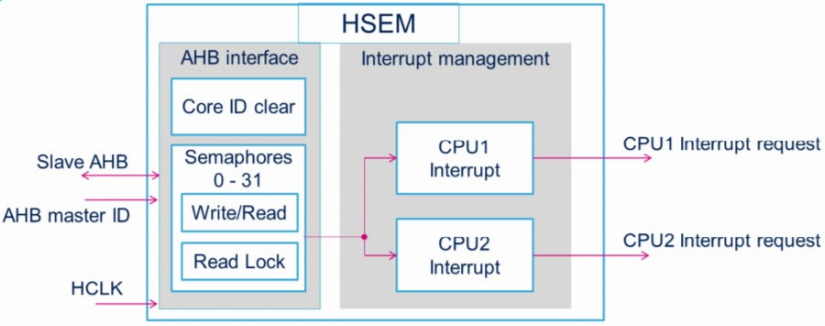
\includegraphics[width=0.6\textwidth]{images/Multicore/hw_semaphores}

